
% !TEX root = NotesDeCours.tex





\begin{frame}

  \color{bleu}

  \begin{flushleft}
    
    \Large
   	\bf
    
    Mécanique des fluides 

  \end{flushleft}
  
  \ligne{3} % remplace: \noindent \thickline{0.5mm}{150}

  \begin{flushright}

    \rm

    \textrm{David} \textsc{Fabre}
    
    \vspace{3mm}
    
    IMFT / UPS
    
    Département de Mécanique
    
  %  brancher@imft.fr

  \end{flushright}

\begin{picture}(110, 22)(-9, 5)
  \put( 0, 25){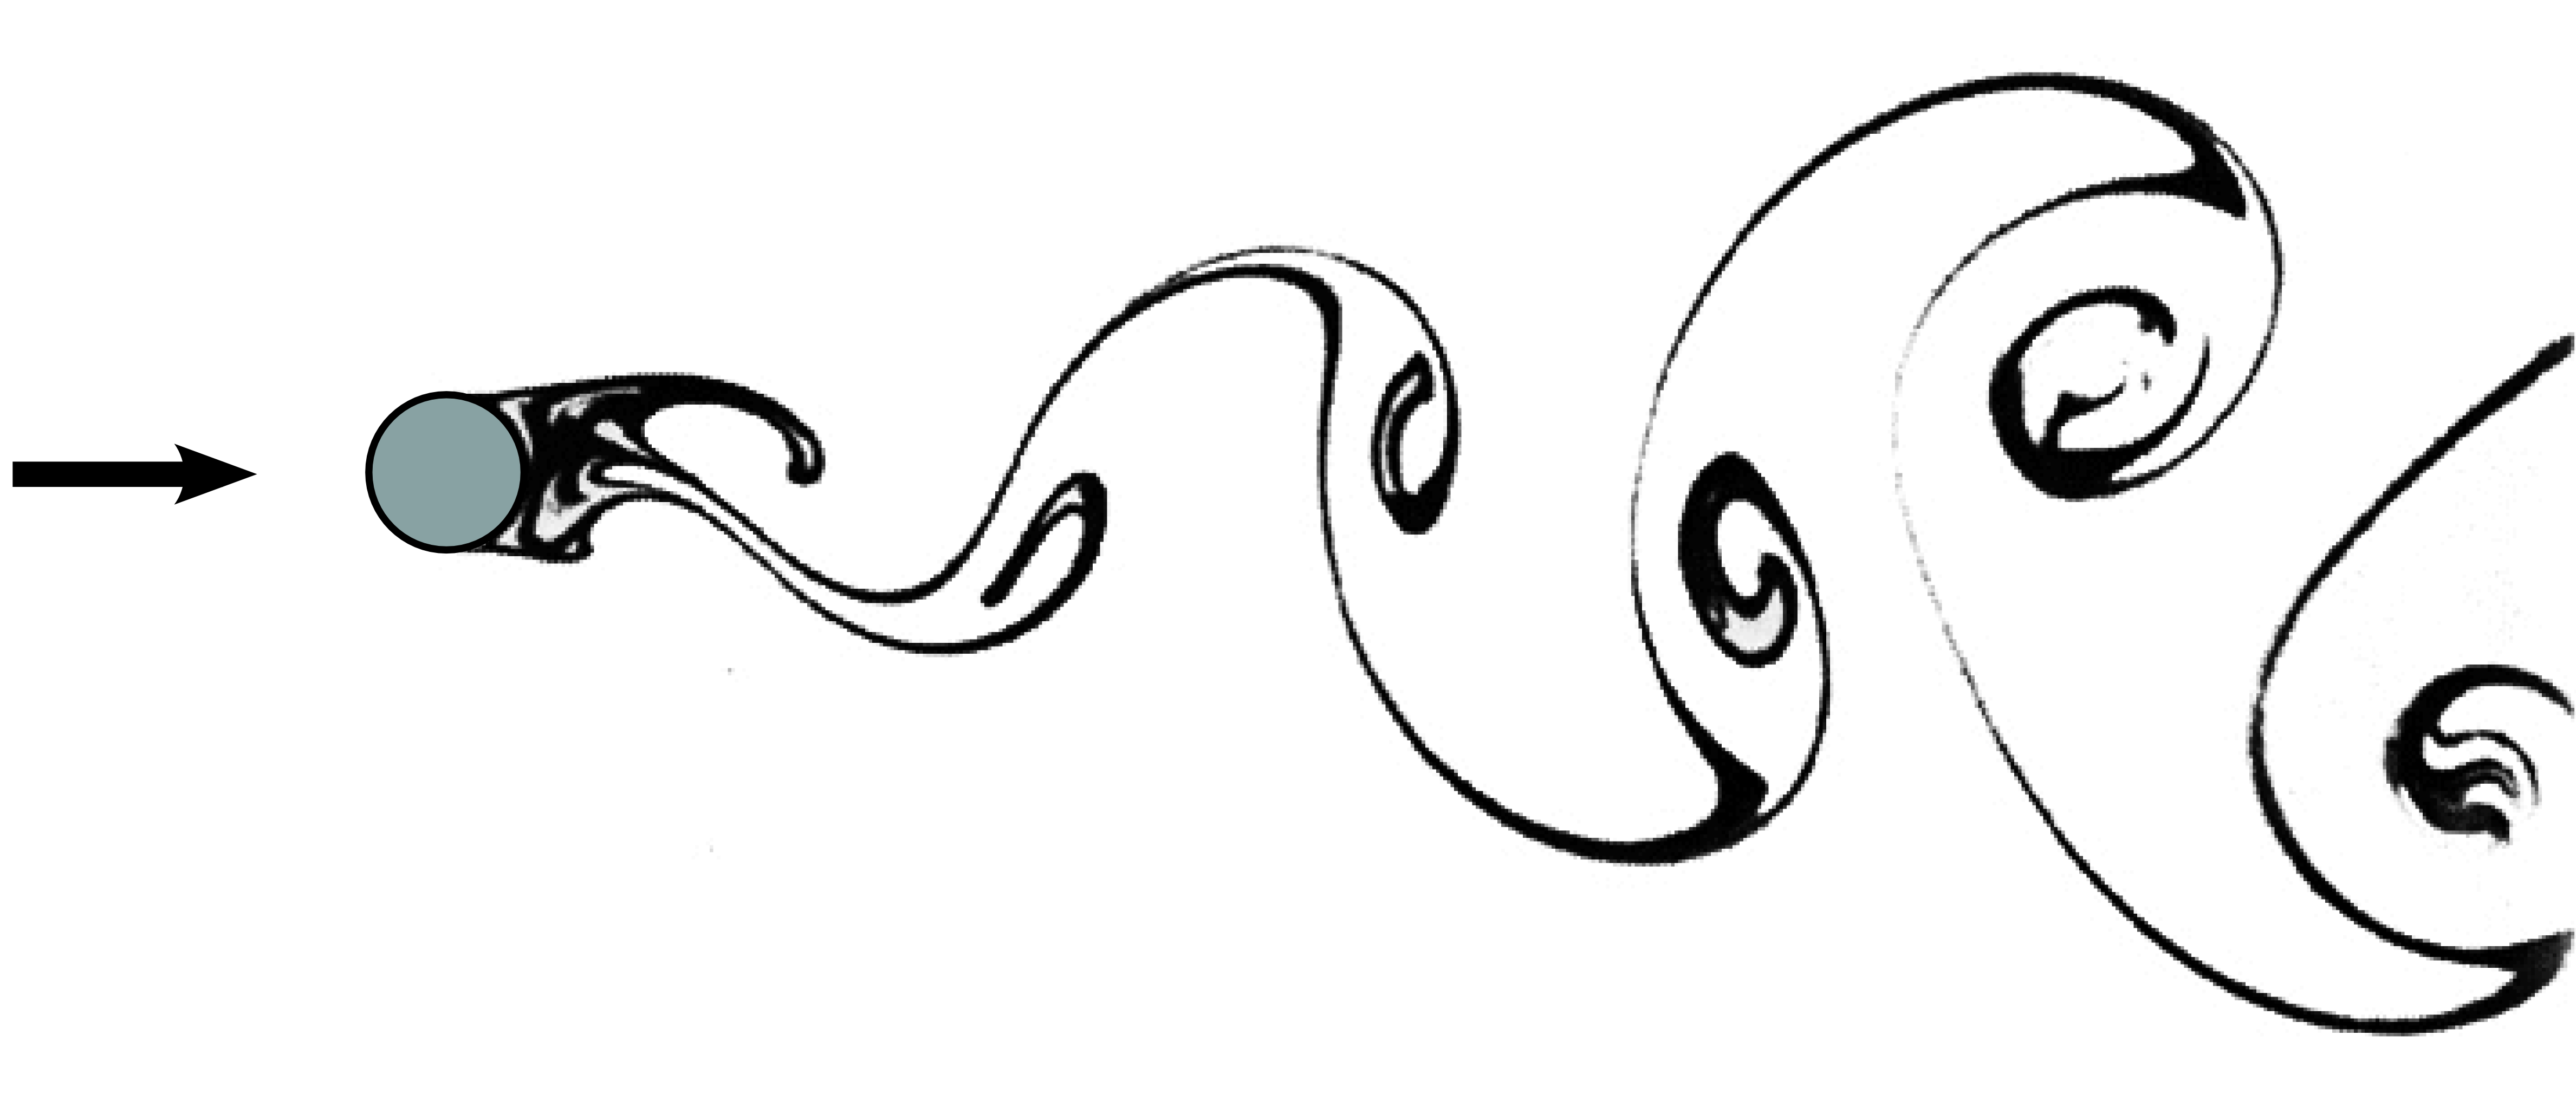
\includegraphics[width=50mm]{./Figures/Von_Karman.png}}
  \put( 6,  0){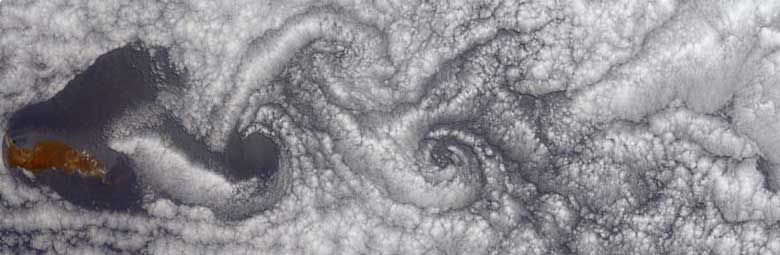
\includegraphics[width=50mm]{./Figures/VK_Guadalupe.jpg}}
  \put( 0, 23){\color{gris} \small \rm Allée de tourbillons de Von Karman} 
  \put( 0, 20){\color{gris} \small \rm en aval d'un cylindre à $Re=140$ (lignes d'émission).}
  \put( 0,  -3){\color{gris} \small \rm Allée de tourbillons de Von Karman}
  \put( 0, -6){\color{gris} \small \rm dans le sillage de l'île de Guadalupe (océan Pacifique).}
\end{picture}

  \vspace{12mm}
  
  \begin{flushright}
    
    \Large
   	\bf
    
    7. Ecoulements inertiels

  \end{flushright}

\end{frame}

%%%%%%%%%%%%%%%%%%%%%%%%%%%%%%%%%%%%%%%%%%%%%%%%%%%%%%%%%%%%%%%%%%%%%%%%%%%%%%%%%%%%%%%%%%
% Sommaire :
%%%%%%%%%%%%%%%%%%%%%%%%%%%%%%%%%%%%%%%%%%%%%%%%%%%%%%%%%%%%%%%%%%%%%%%%%%%%%%%%%%%%%%%%%%

\part{Ecoulements Inertiels}


\section*{\bfseries 7. Ecoulements inertiels}

%\begin{frame}{Sommaire}
%\small
%  
%\hspace*{2mm}
%\begin{tabular}{cc}
%		%&
%  		\begin{minipage}{62mm}
%  			\tableofcontents
%      \vspace{15mm}
%  		\end{minipage}
%  		&   
%  		\begin{minipage}{60cm}
%		  \vspace*{-5mm}  
%  			%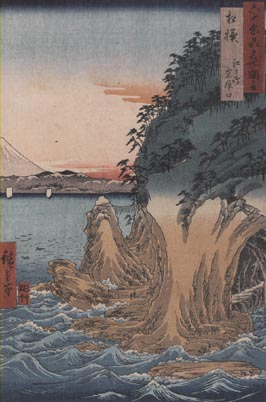
\includegraphics[width=40mm]{vagues.jpg} 
%  		\end{minipage}
%  	\end{tabular}
%
%\vspace{0mm}
%
%\end{frame}

%%%%%%%%%%%%%%%%%%%%%%%%%%%%%%%%%%%%%%%%%%%%%%%%%%%%%%%%%%%%%%%%%%%%%%%%%%%%%%%%%%%%%%%%%%
%\section{\bfseries Ecoulements inertiels}
%%%%%%%%%%%%%%%%%%%%%%%%%%%%%%%%%%%%%%%%%%%%%%%%%%%%%%%%%%%%%%%%%%%%%%%%%%%%%%%%%%%%%%%%%%

%==========================================================================================
\subsection{L'approximation d'écoulement inertiel}
%=========================================================================================

%-----------------------------------------------------------------------------------------
\subsubsection{Définitions}
%-----------------------------------------------------------------------------------------
\begin{frame}{Définitions}
%-----------------------------------------------------------------------------------------

\small

On appelle \textcolor{vert}{écoulement inertiel} tout écoulement pour lequel 
le mode de transport de la quantité \\ de mouvement par advection est dominant 
par rapport au tranport par diffusion visqueuse (frottements).

\medskip
\pause

Dans ces conditions, si $U$ et $L$ désignent les échelles caractéristiques de vitesse 
et de longueur \\ de l'écoulement, le temps caractéristique d'advection de la quantité de mouvement
$\tau_{a} = L/U$ \\
est donc beaucoup plus court que le temps de diffusion 
$\tau_{d} = L^2/\nu$, soit :

\begin{equation}
  \frac{\tau_{d}}{\tau_{a}} = \frac{L^2/\nu}{L/U} \gg 1
  \quad \Rightarrow \quad
  \color{rouge}
  Re \equiv \frac{UL}{\nu} \gg 1
\end{equation}

o\`u $Re$ désigne le \textsl{nombre de Reynolds} :

les écoulements inertiels sont ainsi aussi appelés \textcolor{vert}{écoulements à grand nombre de Reynolds}

\begin{center}
\begin{picture}(40, 30)(0, 0)
	\put(0, 0){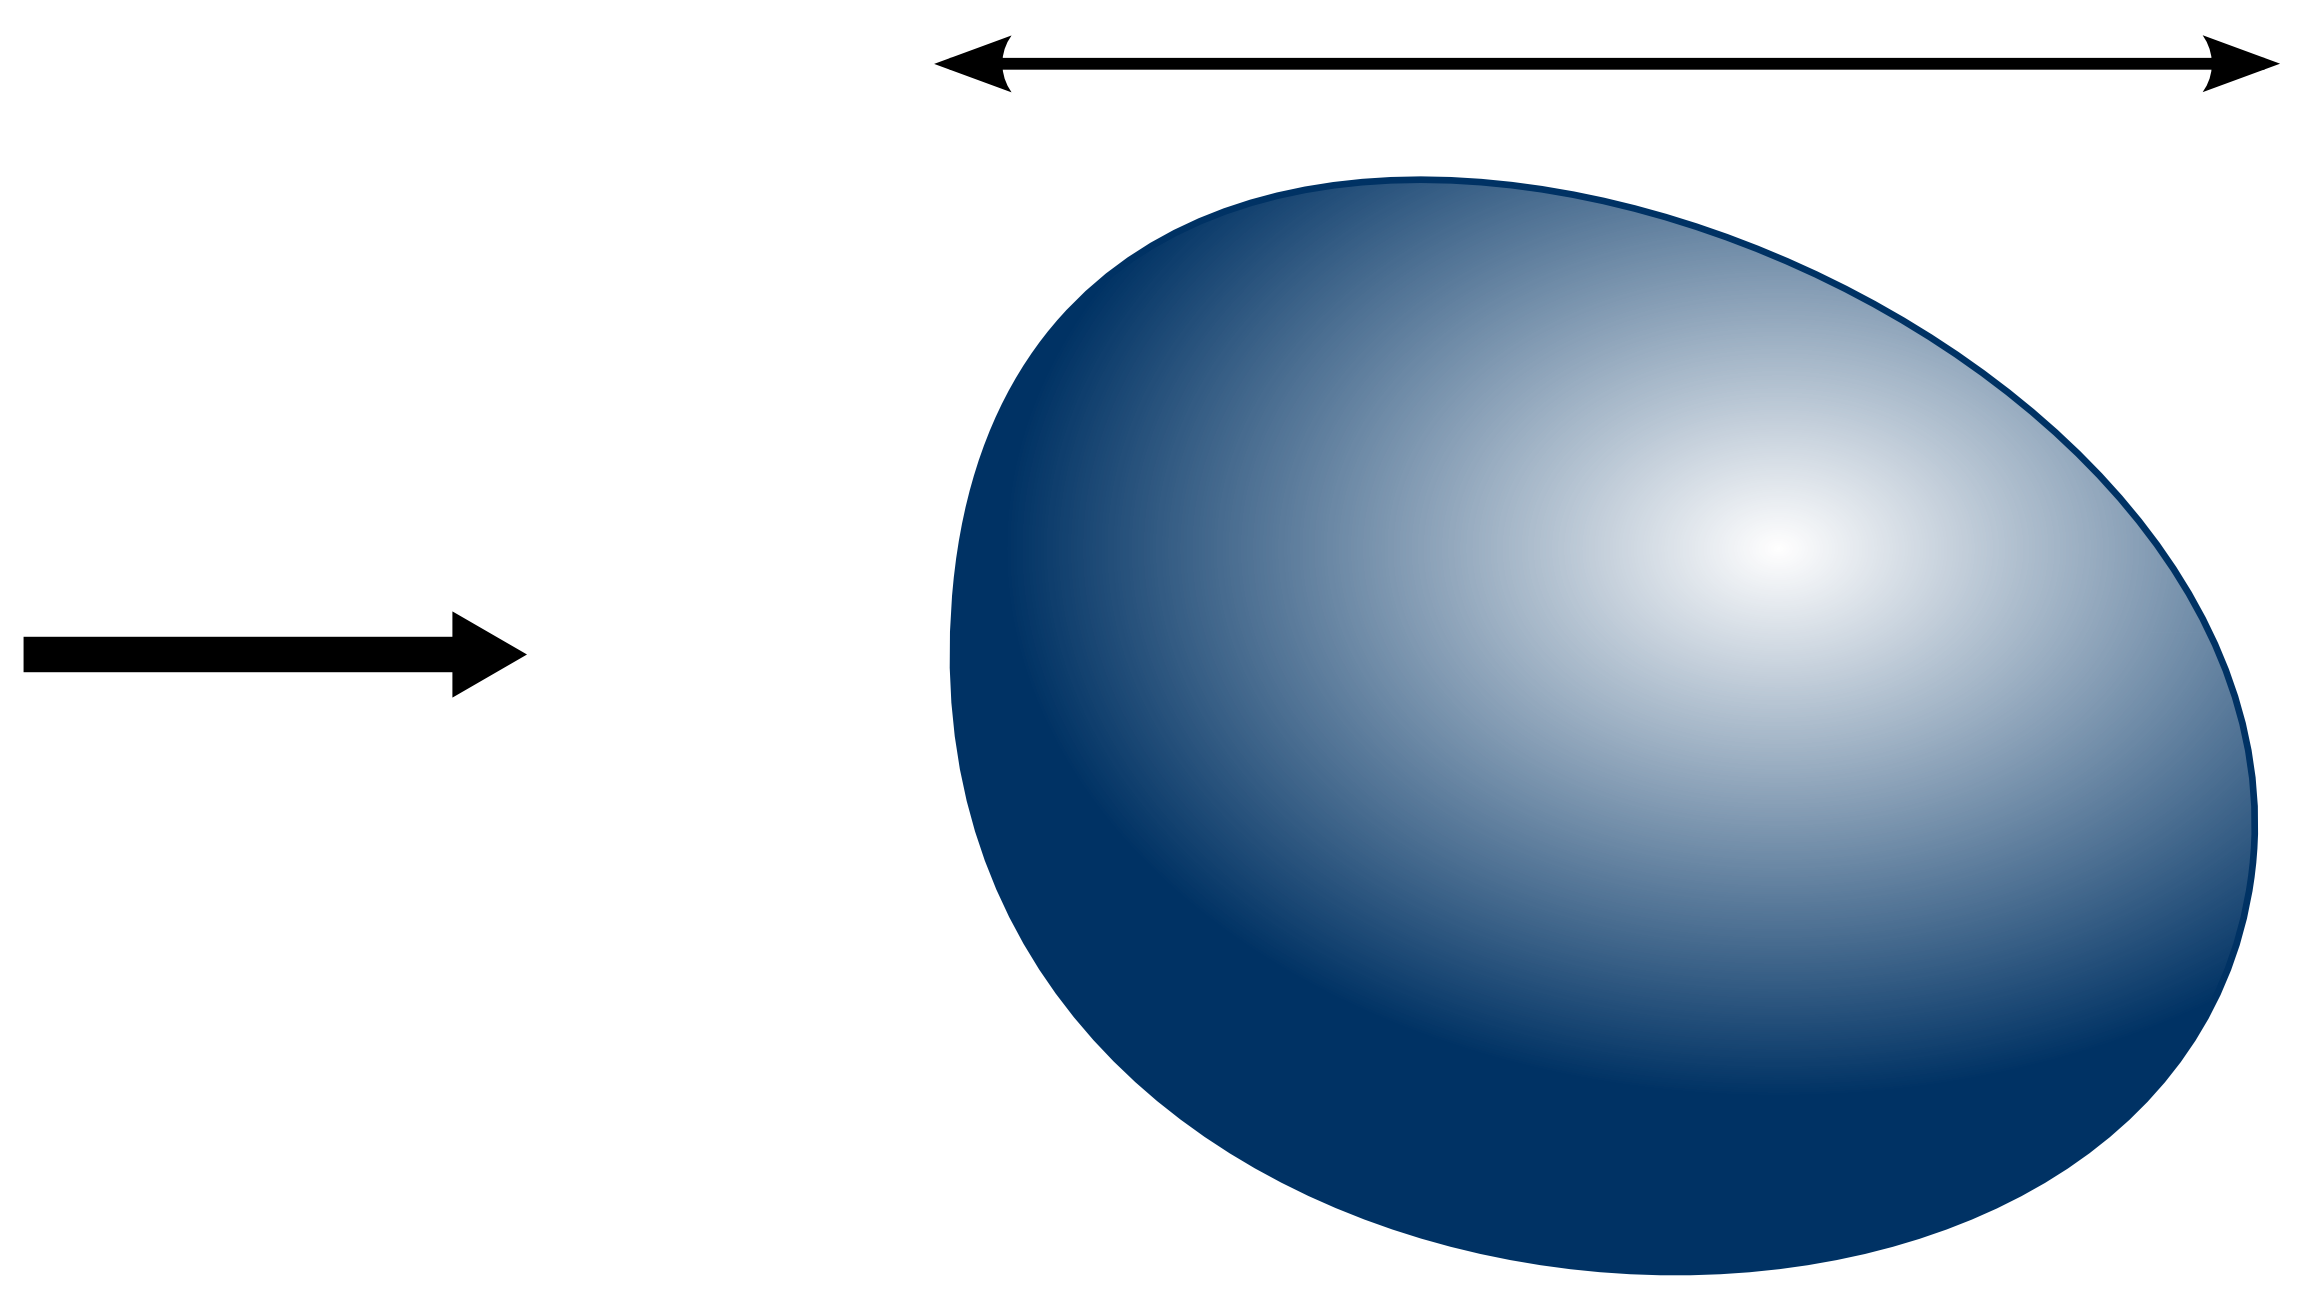
\includegraphics[width=40mm]{obstacle.png}}	
	\put(3, 13){$U$}
	\put(25, 21){\setlength{\fboxsep}{0.5mm}\colorbox{white}{$L$}}
\end{picture}
\end{center}

\vspace{0mm}

\end{frame}

%-----------------------------------------------------------------------------------------
\subsubsection{Exemples}
%-----------------------------------------------------------------------------------------
\begin{frame}{Exemples}
%-----------------------------------------------------------------------------------------

\small

Ecoulements inertiels :
\[
  \color{rouge}
  Re \equiv \frac{UL}{\nu} \gg 1
\]

\pause

\begin{itemize}[<+-| alert@+>]
\item
	Tache rouge de Jupiter : \\
	$U\sim 100$ m/s (360 km/h), $L \sim 15 000$ km, $\nu \sim 15\times 10^{-6}$ m$^2$/s (cf. air) 
	$\Rightarrow \; Re\sim 10^{14}$
\item
	Cyclone : \\
	$U\sim 45$ m/s (170 km/h), $L \sim 100$ km, $\nu \sim 15\times 10^{-6}$ m$^2$/s 
	$\Rightarrow \; Re\sim 3\times 10^{11}$
\item
	Avion : \\
	$U\sim 100$ m/s (360 km/h), $L \sim 15$ m, $\nu \sim 15\; 10^{-6}$ m$^2$/s 
 	$\Rightarrow \; Re\sim 10^{8}$
\item
	Bateau : \\
	$U\sim 10$ m/s (20 noeuds, 36 km/h), $L \sim 10$ m, $\nu \sim 10^{-6}$ m$^2$/s 
	$\Rightarrow \; Re\sim 10^{8}$
\item
	Nageur : \\
	$U\sim 1$ m/s, $L \sim 2$ m, $\nu \sim 10^{-6}$ m$^2$/s 
	$\Rightarrow \; Re\sim 2\times 10^{6}$
\item
	Ballon de foot : \\
	$U\sim 30$ m/s (100 km/h), $L \sim 0.2$ m, $\nu \sim 15 \times 10^{-6}$ m$^2$/s 
	$\Rightarrow \; Re\sim 4\times 10^{5}$
\item
	Robinet : \\
	$U\sim 50$ cm/s, $L \sim 2$ cm, $\nu \sim 10^{-6}$ m$^2$/s 
	$\Rightarrow \; Re\sim 10^4$
\item[]
\end{itemize}

%\pause

\vspace{5mm}

\end{frame}

%==========================================================================================
\subsection{Le modèle de fluide parfait}
%=========================================================================================

%-----------------------------------------------------------------------------------------
\subsubsection{L'équation d'Euler}
%-----------------------------------------------------------------------------------------
\begin{frame}{Equation d'Euler}
%-----------------------------------------------------------------------------------------

\small

Considérons l'écoulement incompressible d'un fluide newtonien homogène (masse volumique uniforme), dans le champ de pesanteur (par ex.).

\pause 

\medskip

L'écoulement vérifie donc l'équation de continuité 
$\divergence \myvec{u} = 0$ et l'équation de Navier--Stokes :
\begin{equation}
  \ddt{\myvec{u}} = \dpdt{\myvec{u}}  + \left( \mytensor{grad} \, \myvec{u} \right) \cdot \myvec{u}
  =
  - \frac{1}{\rho} \, \gradient p + \myvec{g} 
  + \nu \, \Delta \myvec{u}
  =
  - \frac{1}{\rho} \, \gradient \hat{p} 
  + \nu \, \Delta \myvec{u}  
\end{equation}
o\`u $\hat{p} \equiv p - \rho \myvec{g} \cdot \myvec{x} = p + \rho g z$ 
est la pression motrice
($z$ désigne la direction verticale ascendante).

\bigskip

\pause

Le rapport des ordres de grandeur des termes d'inertie à gauche et du terme de diffusif de droite s'écrit
\begin{equation}
  \mbox{\color{gris} [Démonstration] \; $\longrightarrow$ \;}
  \frac{U^2/L}{\nu U/L^2} = \color{rouge}\frac{UL}{\nu} = Re \gg 1
\end{equation}

\pause
\medskip

Le terme visqueux est donc négligeable devant le terme inertiel,
d'o\`u l'\textcolor{vert}{équation d'Euler} :
\begin{equation}
	\color{rouge} 
  \dpdt{\myvec{u}} + \left( \mytensor{grad} \, \myvec{u} \right) \cdot \myvec{u}
  =
  - \frac{1}{\rho} \, \gradient{\hat{p}}
\end{equation}

\vspace{20mm}

\end{frame}

%-----------------------------------------------------------------------------------------
\subsubsection{Ecoulement de fluide parfait}
%-----------------------------------------------------------------------------------------
\begin{frame}{Ecoulement de fluide parfait}
%-----------------------------------------------------------------------------------------

\small

L'équation d'Euler obtenue pour un écoulement inertiel peut être aussi interprétée comme 
l'équation du mouvement pour un fluide "théorique", idéalisé, parfaitement non visqueux, 
c'est-à-dire de viscosité nulle $\nu=0$, appelé \textcolor{vert}{fluide parfait}.

%\hspace{-10mm}
\begin{minipage}{90mm}
\[
	\left .
	\begin{array}{r}
	\dpdt{\myvec{u}} + \left( \mytensor{grad} \, \myvec{u} \right) \cdot \myvec{u}
  =
  - \frac{1}{\rho} \, \gradient \hat{p} 
  + \nu \, \Delta \myvec{u}
  \\
  \nu = 0
  \end{array}
  \right \} 
  \quad \Rightarrow \quad 
	\dpdt{\myvec{u}} + \left( \mytensor{grad} \, \myvec{u} \right) \cdot \myvec{u}
  =
  - \frac{1}{\rho} \, \gradient{\hat{p}} 
\]
\end{minipage}

\bigskip
\pause

Les écoulements inertiels sont donc aussi aussi parfois appelés 
\textcolor{vert}{écoulements de fluide parfait}, même si cette dénomination 
oublie que l'équation d'Euler n'est qu'une simplification de l'équation de Navier--Stokes
dans la limite $Re\gg 1$ et que le fluide parfait n'existe pas 
(tous les fluides ayant une viscosité), a quelques exceptions exotiques près :

- Hélium liquide "superfluide" à $T<4K$ ;

- Condensats de Bose-Einstein

- Plasmas de quarks et gluons (intérieur des étoiles à neutron...)

% sauf les superfluides, ce qui en pratique ne concerne 
%guère que l'hélium à très basse température et peut-être l'intérieur d'une étoile à neutrons).
%
%	\begin{center}
%		\setlength{\unitlength}{1mm}
%		\begin{picture}(90, 35)(5, 0)
%			\put(0, 0){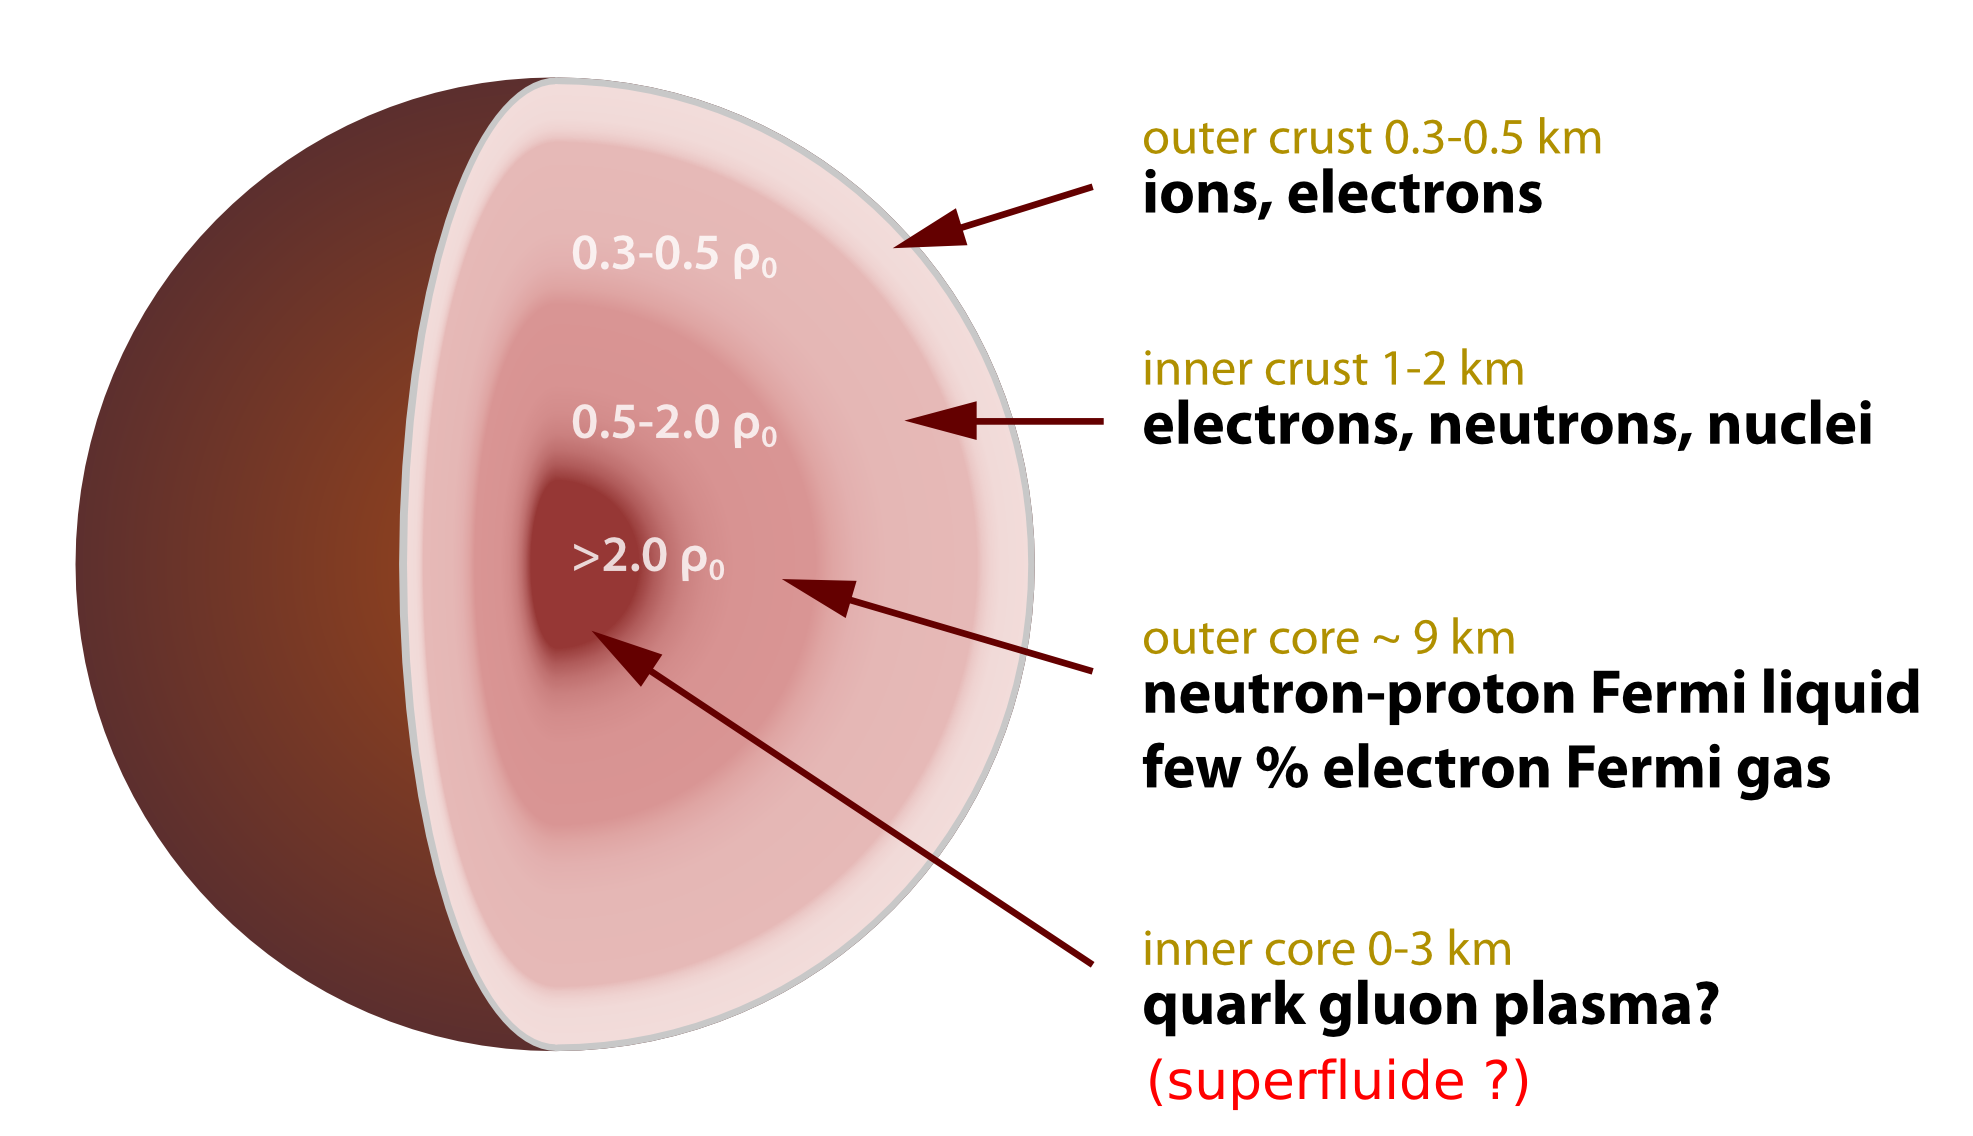
\includegraphics[width=60mm]{Neutron_star_cross_section.png}}	
%			\put(63, 20){\footnotesize \sl Cross-section of a neutron star.} 
%			\put(63, 17.5){\footnotesize \sl Densities are in terms of $\rho_0$,} 
%			\put(63, 15){\footnotesize \sl the saturation nuclear matter density,} 
%			\put(63, 12.5){\footnotesize \sl where nucleons begin to touch.}
%		\end{picture}
%	\end{center}

\vspace{0mm}

\end{frame}




%------------------------------------------------------------------------------------------
\begin{frame}{Propriétés de l'équation d'Euler} \hypertarget{frame:toto}{}
%------------------------------------------------------------------------------------------

\small

L'équation d'Euler n'est pas beaucoup plus facile à résoudre que celle de N-S, et pose quelques problèmes conceptuels...
\pause
\begin{itemize}
\item Dans certains cas elle n'a pas de solution unique (exemple : écoulements parallèles
de la forme $u(y)$)
\pause
\item Elle autorise des solutions discontinues (couches de cisaillement).
\end{itemize}
\pause
Mathématiquement l'équation d'Euler est d'ordre 1 en espace et nécessite donc des conditions limites moins contraignantes que l'équation de Navier-Stokes :

\pause

\vspace{25mm}
	\begin{center}
		\setlength{\unitlength}{0.4mm}
		\begin{picture}(65, 50)(12, -12)
			\put(0, 0){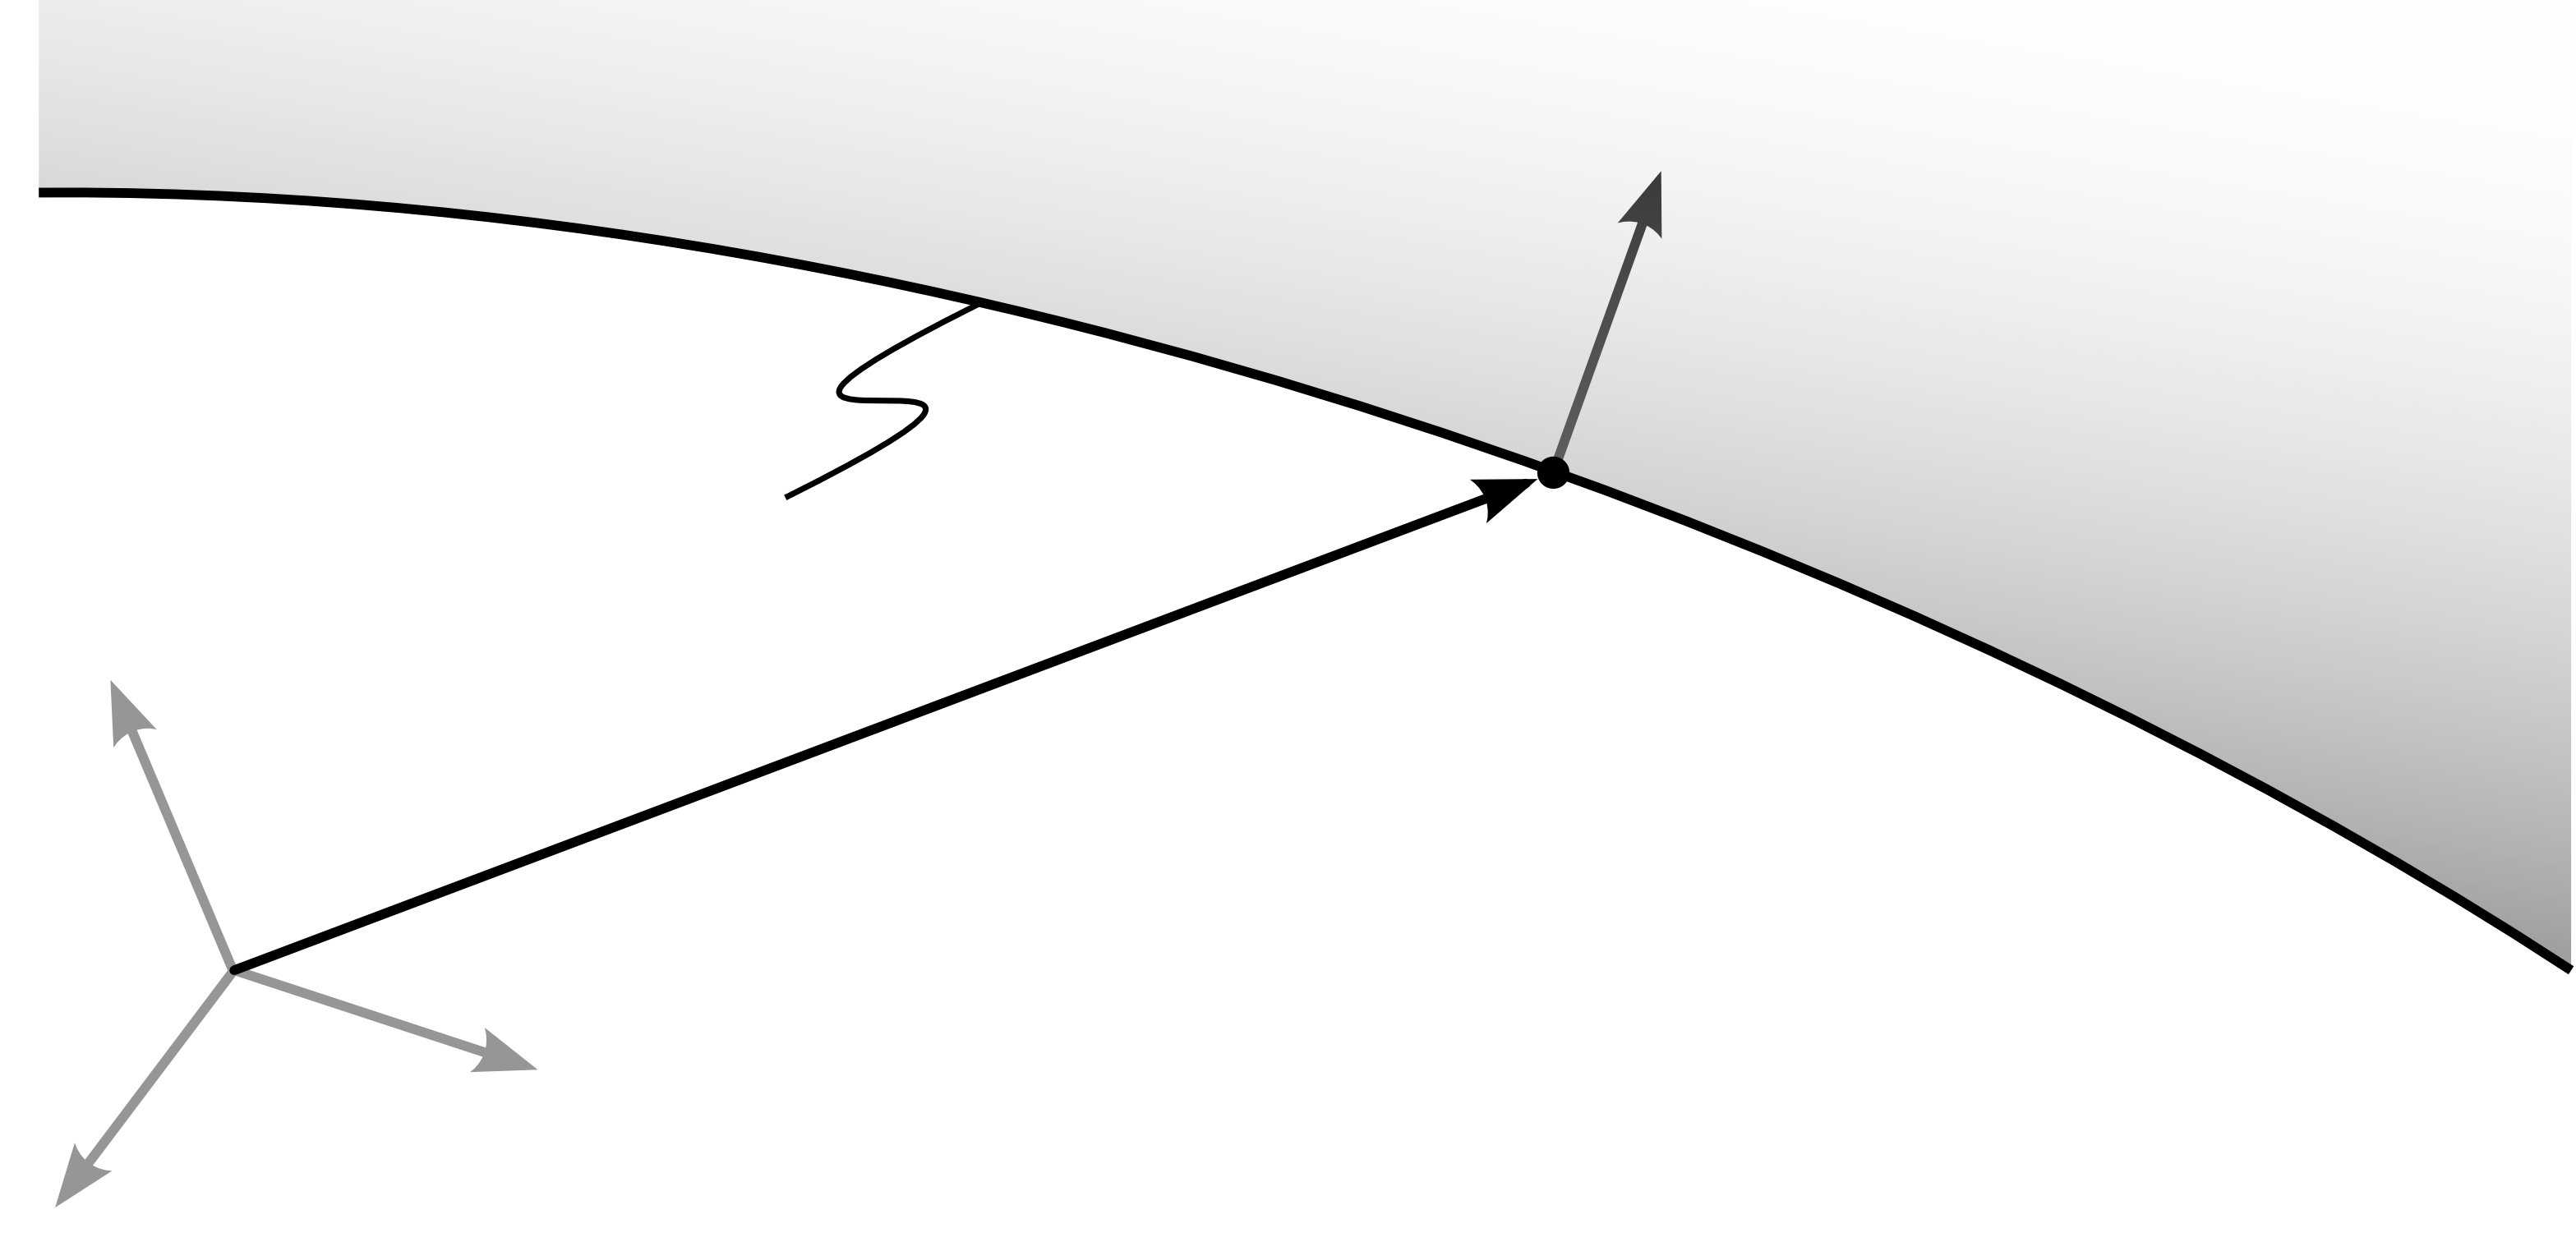
\includegraphics[width=63mm]{conditions_limites.png}}	
			\put(88, 59){$\myvec{n}$}
			\put(93.5, 52){milieu extérieur}
			\put(93, 47){(paroi solide)}
			\put(58, 37){\setlength{\fboxsep}{1mm}\colorbox{white}{$\myvec{x}$}} 
			\put(39, 44){\color{rouge} frontière $\Sigma$}
			\put(93, 35){fluide}
		\end{picture}
	\end{center}



\vspace{-8mm}

\begin{tabular}{cl}
fluide réel 
&
continuité de la vitesse (condition d'adhérence)
\\
(visqueux) &
$\color{bleu}\myvec{u}(\myvec{x} \in \Sigma, t) = \myvec{u}\indice{ext}(\myvec{x} \in \Sigma, t)$
\\
\\
\color{rouge} 
fluide parfait 
&
continuité de la vitesse \textcolor{rouge}{normale} (condition de glissement ou non-pénétration)
\\
(non visqueux) & 
$\color{bleu}\myvec{u}(\myvec{x} \in \Sigma, t){\color{rouge}\cdot \myvec{n} }
= 
\myvec{u}\indice{ext}(\myvec{x} \in \Sigma, t){\color{rouge}\cdot  \myvec{n}}$
\end{tabular}

\vspace{0mm}

\end{frame}

%
%%-----------------------------------------------------------------------------------------
%\subsubsection{Force exercée sur un obstacle}
%%-----------------------------------------------------------------------------------------
%\begin{frame}{Force exercée sur un obstacle}
%%-----------------------------------------------------------------------------------------
%
%\small
%%
%%Pour des obstacles de forme générale, d'échelle de longueur
%%caractéristique donnée $L$, l'équation d'Euler permet de remonter à l'ordre 
%%de grandeur des variations de pression
%%dans un écoulement inertiel :
%%\begin{equation*}
%%	\color{rouge} 
%%  \underbrace{\ddt{\myvec{u}} = \dpdt{\myvec{u}} + \left( \mytensor{grad} \, \myvec{u} \right) \cdot \myvec{u}}_{\displaystyle U^2/L}
%%  =
% % \underbrace{- \frac{1}{\rho} \, \gradient p}_{\displaystyle \Delta P / (\rho L) }
% % \quad \Rightarrow \quad
% % \Delta P = \rho \, U^2
%%\end{equation*}
%
%%\medskip
%
%Estimation qualitative de la force de traînée exercée sur un obstacle non profilé.
%
%\begin{center}
%	\begin{picture}(40, 25)(0, 0)
%		\put(0, 0){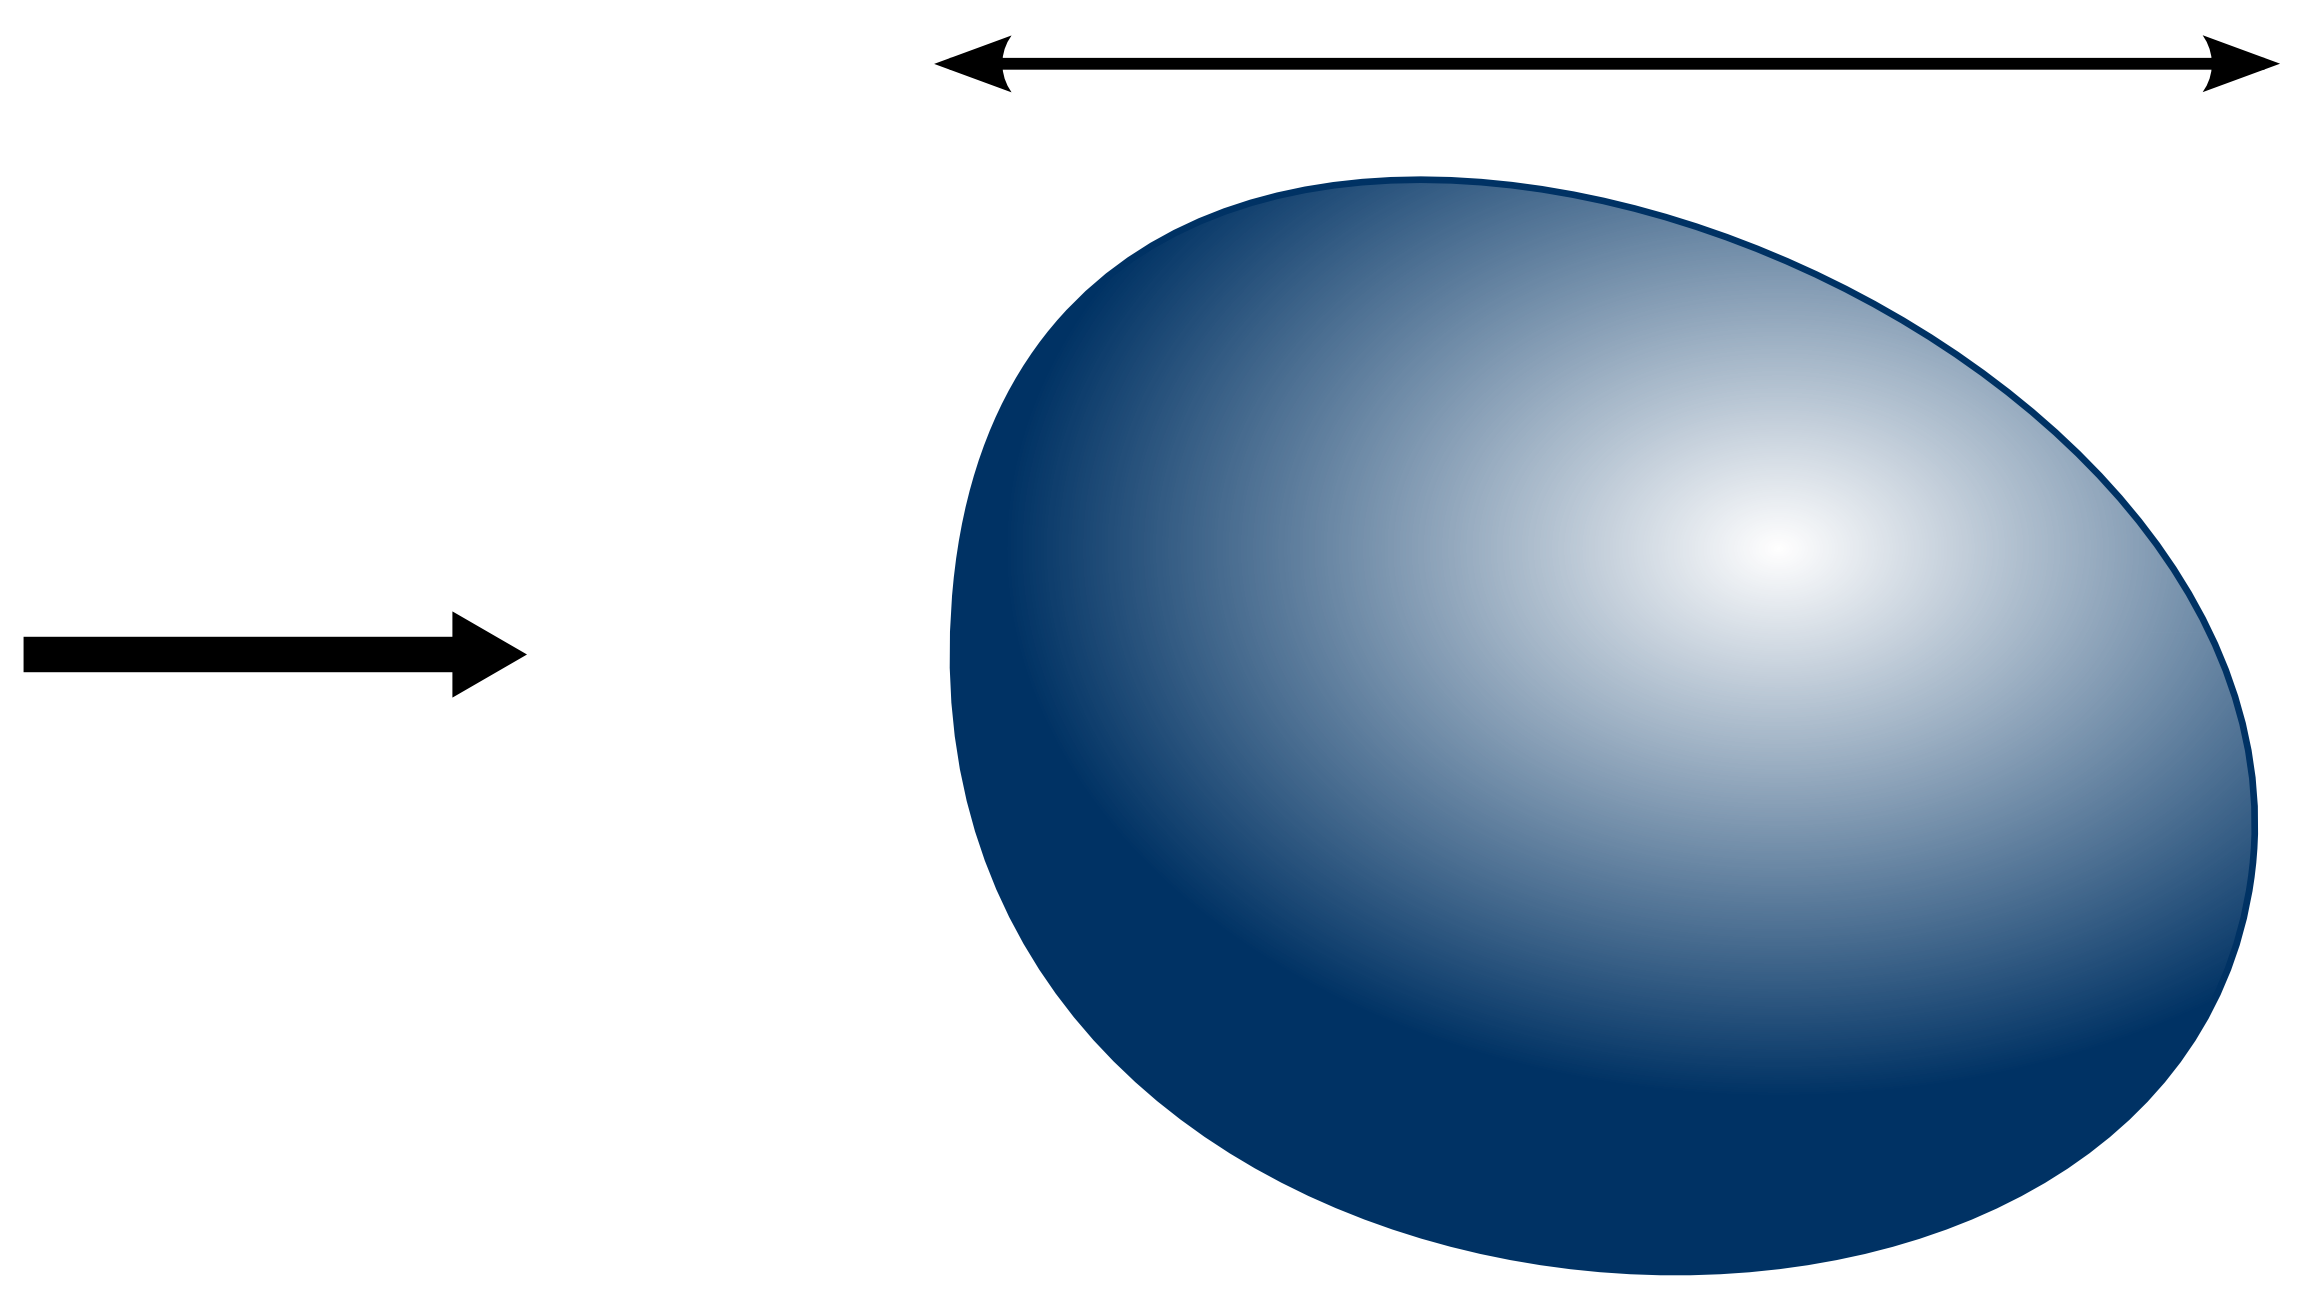
\includegraphics[width=40mm]{obstacle.png}}	
%		\put(3, 13){$U$}
%		\put(25, 21){\setlength{\fboxsep}{0.5mm}\colorbox{white}{$L$}}
%		\put(27, 10){\color{rouge}\vector(1, 0){20}}
%		\put(49, 9.5){\color{rouge}$F \sim \rho L^2 U^2$}
%	\end{picture}
%\end{center}
%
%
%Dans le régime inertiel, on observe de manière assez générale l'existence d'une zone de recirculation derrière l'objet dont la structure ne dépend plus de $Re$ si celui-ci est suffisamment grand.
%
%
%
%\begin{itemize}
%\item $ p \approx p_0 + \rho U^2/2$ (pression d'arrêt) sur la face amont de l'objet 
%
%\item $ p \approx p_0$ (pression statique) sur la face aval de l'objet (zone de recirculation).
%\end{itemize}
%
%D'où une force résultante d'ordre 
%\[
%	\color{rouge} F \sim \Delta P \times S \sim \rho U^2 L^2
%\]
%
%Pour la traînée : \qquad
%$	{\color{rouge}  F_x  =\frac{\rho S U^2}{2} C_x( {\cal G}_i)}  $
%
%\medskip 
%\pause 
%
%$\rightarrow $ A haut $Re$ le $C_x$ ne dépend que de la géométrie de l'objet.
%
%\medskip 
%\pause 
%
%Exemples : 
%
%Sphère $C_x\approx 0.44$  ( dans la gamme $10^3 <Re < 5 \cdot 10^5$)
%
%Disque $C_x \approx 0.8$ ( $Re > 10^3$)
%
%Automobile $0.22 < C_x  < 0.38$
%
%Aile d'avion $C_x = C_x (\alpha) \approx 0.1 + k \alpha^2$ 
%
%



%A comparer avec le cas de la force de Stokes pour les écoulements visqueux $F \sim \mu U L$\ldots


%\vspace{5mm}

%\end{frame}



\subsection{Théorèmes locaux}

%-----------------------------------------------------------------------------------------
\subsubsection{Equation-bilan pour l'énergie cinétique}
%-----------------------------------------------------------------------------------------
\begin{frame}{Equation pour l'énergie cinétique}
%-----------------------------------------------------------------------------------------

\small

Repartons de l'équation de Navier-Stokes pour un fluide homogène de masse volumique $\rho$ soumis à une force extérieure volumique $\vec f$ : 
\begin{equation}
	\color{rouge}
  \dpdt{\myvec{u}} + \left( \mytensor{grad} \, \myvec{u} \right) \cdot \myvec{u}
  =
  -\frac{1}{\rho} \gradient p + \vec{f}  + \nu \Delta  \myvec{u}.
\end{equation}
%si l'on tient compte de la pesanteur $g$ ($z$ correspond à la verticale ascendante).

\medskip \pause

En notant $\myvec{\omega} = \rot(\myvec{u})$ le champ de vorticité et 
$u^2 = ||\myvec{u}||^2$, utilisons l'égalité mathématique (à vérifier en exercice)
\begin{equation*}
 \left( \mytensor{grad} \, \myvec{u} \right) \cdot \myvec{u}
  =
  \myvec{\omega} \wedge \myvec{u} + \frac{1}{2} \gradient{u^2}
\end{equation*}
%permet d'écrire l'équation d'Euler sous la forme 
%\begin{equation*}
 % \dpdt{\myvec{u}} + \myvec{\omega} \wedge \myvec{u} + \gradient \left ( \frac{1}{2} u^2 \right )
 % = 
  %- \gradient \left ( \frac{p}{\rho} + gz \right )
%\end{equation*}

\medskip \pause

En prenant le produit scalaire de l'eq. de Navier-Stokes avec $ \myvec{u}$, on obtient
l'équation de bilan local pour l'énergie cinétique {\em massique}
$\displaystyle e_k = \frac{1}{2} u^2$ :

\bigskip

\begin{equation}
  \mbox{\color{gris} [Démonstration] \; $\longrightarrow$ \;}
	\color{rouge}
  \ddt{e_k} = \dpdt{e_k} + \myvec{u}\cdot \gradient \left (e_k\right)
  = 
  - \myvec{u} 
  \cdot \frac{\gradient p}{\rho}  + \vec{f} \cdot \vec{u} + \rho \Pi_v 
\end{equation}

où $\Pi_v = (1/\rho) \myvec{div}({\mytensor{\tau}}) \cdot \myvec{u}$ est la puissance massique des efforts visqueux.

\medskip

\pause

Si $\vec f = -g \vec{e}_z$ et si le fluide est incompressible ($\rho$ est uniforme),
On peut réécrire ce bilan en introduisant l'énergie mécanique massique : 
$e_m \equiv p/\rho  + g z + \frac{1}{2} u^2 $ :


\begin{equation}
  \mbox{\color{gris} [Démonstration] \; $\longrightarrow$ \;}
	\color{rouge}
  \ddt{e_m} = \dpdt{e_m} + \myvec{u}\cdot \gradient \left (e_m\right)
  = 
\frac{1}{\rho} \frac{\partial p}{\partial t} + \Pi_v 
\end{equation}

\pause
\medskip
\small

Remarque : on peut décomposer $\Pi_v$ en puissance extérieure et puissance intérieure 
 $\rho \Pi_v = \myvec{div}({\mytensor{\tau}}) \cdot \myvec{u} 
=  \myvec{div}({\mytensor{\tau}} \cdot \myvec{u} )
- \mytensor{\tau} \cdot  \mytensor{grad} (\myvec{u}) 
\qquad \mbox{ (cf. cours MMC) }
$ 


\vspace{0mm}

\end{frame}



\subsubsection{Premier théorème de Bernoulli}


%-----------------------------------------------------------------------------------------
%\subsubsection{Conservation de l'énergie mécanique}
%-----------------------------------------------------------------------------------------
\begin{frame}{Premier théorème de Bernoulli : conservation de l'énergie mécanique}
%-----------------------------------------------------------------------------------------

\small

On en déduit donc le \textcolor{vert}{Premier théorème de Bernoulli} :
\medskip

Hypothèses : 

$(a)$ fluide incompressible (ou écoulement isovolume),

$(b)$ force volumique $\myvec g = - g \myvec{z} $ uniforme,

$(c)$ écoulement stationnaire,

$(d)$ " Fluide parfait" (ou plus rigoureusement forces visqueuses négligeables),

\smallskip

Alors la quantité 
%\smallskip
%\begin{equation}
$ e_m \equiv p/\rho  + g z + \frac{1}{2}  u^2$ se conserve le long de chaque ligne de courant (ou trajectoire).
%\end{equation}

\medskip
\pause

On note aussi (formellement) : 

$$ 
e_m = C(\myvec{X_0}), \mbox{ où } \myvec{X_0} \mbox{ est le "label" de chaque trajectoire lagrangienne.}
$$



\bigskip \pause

%Ce premier théorème de Bernouilli
%signifie donc que 
%(somme d'une énergie potentielle de pression, de l'énergie potentielle de pesanteur et de l'énergie cinétique) par unité de volume,
%ce premier théorème de Bernoulli traduit la conservation de l'énergie %
%mécanique le long des lignes de courant (ou des trajectoires, ces deux familles
%de courbes étant confondues dans le cas stationnaire) : 
%\begin{center}
%	\color{rouge}
%	les particules fluides conservent leur énergie mécanique.
%\end{center}

%\vspace{9mm}

\bigskip
\pause

Remarques 

\begin{itemize}


\item Dans le cas des gaz on néglige habituellement l'energie potentielle de gravité.

Le théorème de Bernouilli s'écrit alors : $p+ \frac{1}{2} \rho u^2 \equiv p_A = C^{te}$.

$p_A$ est appelée la pression de stagnation ou pression d'arrêt.
  \pause
\item Dans le cas des liquides,  $e_m$ est aussi courrament appelée la charge de l'écoulement.

%Le théorème s'écrit aussi sous la forme :
%$z  + p/(\rho g) /+ u^2/(2g) =  C^{te}(\myvec{X_0})$

\pause
\item Si l'hypothèse $(b)$ est remplacée par 

$(b')$ : Forces volumiques conservatives  $\myvec g = - \gradient {\cal U} $ , 

alors le théorème se généralise en :  
$p + \rho {\cal U} + \frac{1}{2} \rho u^2  = C(\myvec{X_0})$. 
\pause
\item Il existe une généralisation si l'hypothèse $(a)$ est remplacée par 
$(a')$ : Fluide Barotrope,
c.a.d. $\rho = \rho(P)$ (démo en exercice).

\end{itemize}


\end{frame}


\subsubsection{Applications de Bernoulli}

%-----------------------------------------------------------------------------------------
\begin{frame}{Application classiques de Bernoulli}
%-----------------------------------------------------------------------------------------

\begin{enumerate}
\item Tube de Pitot (ou Antenne de Prandtl)

\small
$$
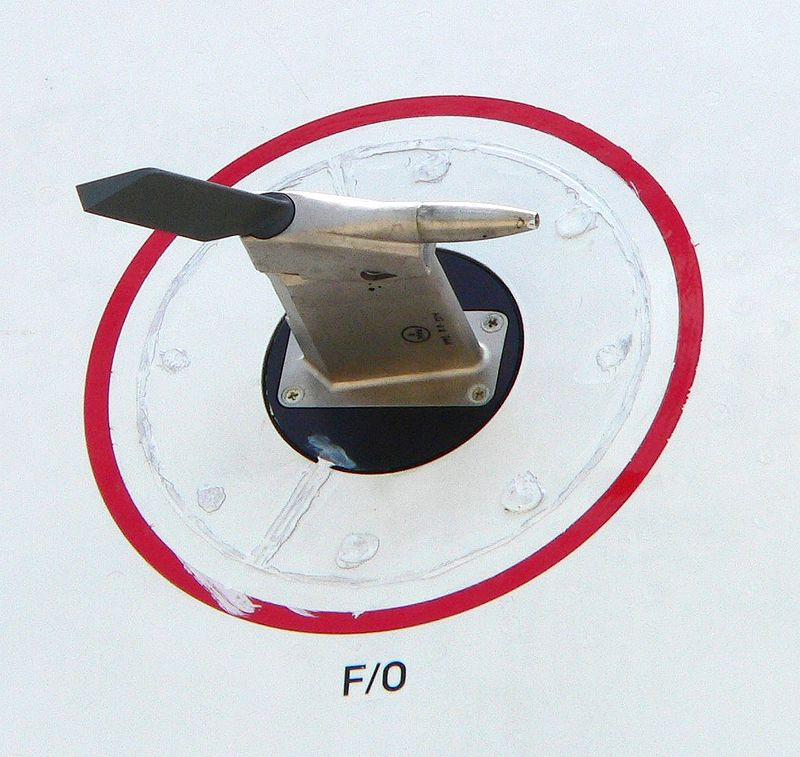
\includegraphics[width=20mm]{Figures/Pitot_A380.jpeg}
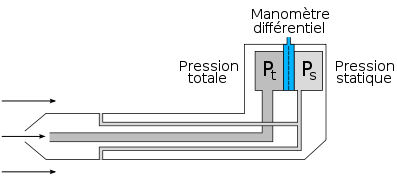
\includegraphics[width=30mm]{Figures/Pitot_principe.png}
$$
\vspace{0mm}


\item Effet Venturi (TP)

\item Loi de Torricelli (Exercice complémentaire)
\end{enumerate}

\end{frame}



\comment{
%-----------------------------------------------------------------------------------------
\subsubsection{Les limites du modèle de fluide parfait}
%-----------------------------------------------------------------------------------------
\begin{frame}{Limites du modèle de fluide parfait}
%-----------------------------------------------------------------------------------------

\small

L'approximation de fluide parfait présente des limites : \pause

\begin{itemize}[<+-| alert@+>]
\item
Le fluide parfait $\nu = 0$ n'existe (pratiquement) pas !
\item
Observations expérimentales : même à $Re\gg 1$, c'est-à-dire pour une viscosité aussi petite 
que l'on veut, on observe que \textcolor{vert}{le fluide adhère à la paroi !}

\smallskip
$\rightarrow$ les conditions aux limites du fluide réel sont \textsl{incontournables}
\end{itemize}

\medskip

\pause

Plus précisément, les observations expérimentales montrent que la condition limite d'adhérence
est assurée à travers d'une couche très fine en proche paroi, en dehors de laquelle
l'écoulement vérifie bien l'équation d'Euler, mais à travers laquelle les frottements visqueux
ne sont plus négligeables. 

\medskip
Cette \textcolor{vert}{couche limite} permet d'assurer l'adhérence.

\begin{overprint}

\onslide<3->

\begin{center}
	\setlength{\unitlength}{1mm}
	\begin{picture}(90, 40)
		\put(0, 5){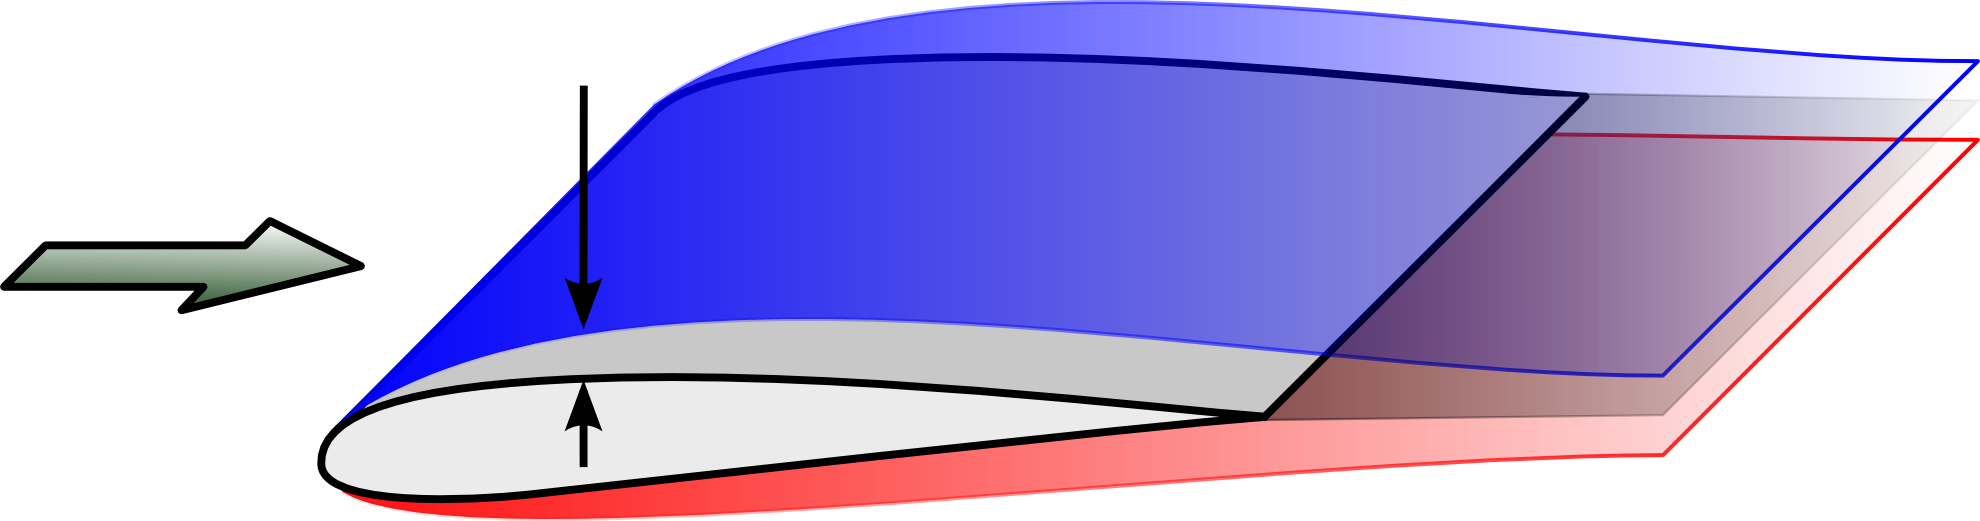
\includegraphics[width=60mm]{couche_limite_airfoil.png}}	
		\put(2, 23){couche limite}
		\put(2, 20){d'épaisseur $\delta \ll L$}
		\put(37, 30){\color{bleu} \vector(-1, -1){5}}
		\put(37,  4.5){\color{rouge} \vector(-1, 1){5}}
		\put(38, 3){\color{rouge} frottements visqueux non négligeables}
		\put(38, 29.5){\color{bleu} frottements visqueux négligeables : Euler OK}
		\put(30, 9.3){\color{rouge} $\bullet$}
		\put(30, 24){\color{bleu} $\bullet$}
		\put(30, 1){\vector(-1, 0){20}}
		\put(30, 1){\vector(1, 0){10}}
		\put(23, 0){\colorbox{white}{$L$}}
	\end{picture}
\end{center}

\end{overprint}

\vspace{0mm}

\end{frame}
}




%-----------------------------------------------------------------------------------------
\subsubsection{Equations intrinsèques}
%-----------------------------------------------------------------------------------------
\begin{frame}{Equations intrinsèques }
%-----------------------------------------------------------------------------------------

\small



\begin{minipage}{55mm}
	%En notant $\hat{p} = p+\rho g z$ la pression motrice, l'équation d'Euler peut aussi s'écrire
	%\begin{equation*}
	 % \rho \ddt{\myvec{u}} = - \gradient{\hat{p}}
	  %\label{eq:euler}
	%\end{equation*}
	%\pause
	Considérons l'écoulement {\em stationnaire} et {\em incompressible} d'un fluide 
	%{\em parfait} $\nu \approx 0$) 
	%{\em non pesant} ($g=0$) 
	dans le régime inertiel ($Re \gg 1$).
	
	En notant $s$ l'abscisse curviligne le long de la ligne de courant,
	$R$, $\myvec{\tau}$ et $\myvec{n}$ respectivement le rayon de courbure, la tangente et la normale
	localement à la ligne de courant (repère de Frenet),
	on montre :
	
\end{minipage}

\setlength{\unitlength}{0.5mm}
\begin{picture}(0, 0)(-115, 17)
	\put(10, 10){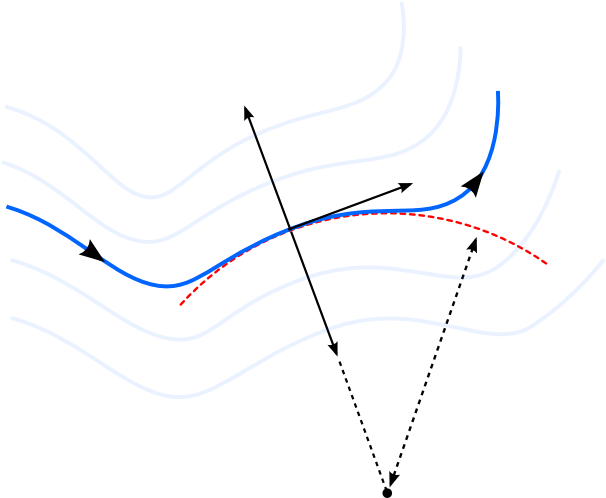
\includegraphics[height=3.3cm]{streamlines.png}}
	\put(67, 10){$C$ \footnotesize (centre de courbure)}
	\put(64, 24.2){\setlength{\fboxsep}{0.5mm}\colorbox{white}{$R$}}
	\put(66, 52){$\myvec{\tau}$}
	\put(53, 24.2){\setlength{\fboxsep}{0.5mm}\colorbox{white}{$\myvec{n}$}}
	\put(40, 65){$r$}
	\put(33, 46){$M(s)$}
	\put(47, 44.5){$\bullet$}
	\put(79, 59){\sl \footnotesize ligne de courant}
\end{picture}

\pause

1/ En projection sur la tangente $\myvec{\tau}$, l'équation d'Euler donne
\begin{equation*}
  \mbox{\color{gris} [Démonstration] \; $\longrightarrow$ \;}
   \frac{\partial}{\partial s} 
   \left ( \frac{1}{2}\rho u^2 + p + \rho g z \right )
   = 0 
\end{equation*}
On retrouve donc une démonstration alternative du 
théorème de Bernoulli  vu précédemment. 
%\begin{equation*}
 %  \frac{\partial}{\partial s} 
  % \left ( \frac{1}{2}\rho u^2 + p + \rho g z \right )
   %= 0 
   %\quad \Leftrightarrow 
   %\quad \color{rouge}
   %\frac{1}{2}\rho u^2 + p + \rho g z = C^{te} \quad
   %\mbox{le long d'une ligne de courant.}
%\end{equation*}

\pause

\smallskip

2/ En projection sur la normale $\myvec{n}$, l'équation d'Euler
donne
\[
  \mbox{\color{gris} [Démonstration] \; $\longrightarrow$ \;}
  \frac{\partial \hat{p}}{\partial n} = - \rho \frac{u^2}{R}
  \quad \mbox{ou encore} \quad
  \color{rouge}
  \frac{\partial \hat{p}}{\partial r} = \rho \frac{u^2}{R}
\]
en notant $r$ la coordonnée locale normale à la ligne de courant, pointant
dans la direction \textsl{oppposée} au centre de courbure (cf. figure). 

\pause

\medskip

{\bf Corollaires  :}

\begin{itemize}

\item 
%\color{vert}
Dans des régions de l'écoulement o\`u les lignes de courant sont rectilignes et parallèles 
($R=\infty$), alors la pression motrice $\hat{p}$ est \textsl{constante perpendiculairement aux lignes de courant}. 

\item Dans des zones de l'écoulement où la vitesse est faible, $\hat{p}$ est {\bf uniforme}.
\end{itemize}

\pause

\smallskip

{\bf Conséquence importante :}

Dans les {\em zones de recirculation} courramment rencontrées dans le sillage d'objets non profilés, la pression (motrice) est uniforme et approximativement égale à la pression "loin de l'objet". 


\vspace{0mm}

\end{frame}


\subsection{Théorèmes intégraux}




%-----------------------------------------------------------------------------------------
\subsubsection{Motivation}
%-----------------------------------------------------------------------------------------
\begin{frame}{Théorèmes intégraux : motivation }
%-----------------------------------------------------------------------------------------

\small

Problème générique : calcul de la force exerçée par un fluide ${\cal F}$ sur une structure
de surface $\Sigma$.

\begin{itemize}[<+->]
\item[]
	Méthode directe : 
	$$ \vec{F}_{{\cal F} \rightarrow \Sigma}   = \oint_\Sigma \left( -p \vec{n} + \mytensor{\tau}\cdot \vec{n} \right) dS  
	$$ 
	\medskip
\item[] 
	Nécessite la connaissance du champ de pression et de contrainte visqueuse sur la surface... pas toujours possible !
	\\
	\begin{picture}(0, 0)(-5, 51)
		\put(0, 0){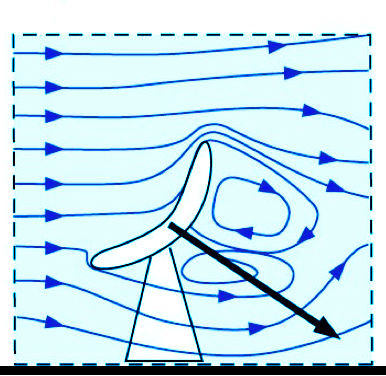
\includegraphics[height = 30mm]{telescope_direct_blue.png}}
	\end{picture}
\item[]
	Alternative ? 
	\medskip
\item[]
	$\rightarrow$  Bilan intégral de quantité de mouvement dans un volume de contrôle 
	\mytabbing{$\rightarrow$} bien choisi\ldots
	\\
	\begin{picture}(0, 0)(-50, 35)
		\put(0, 0){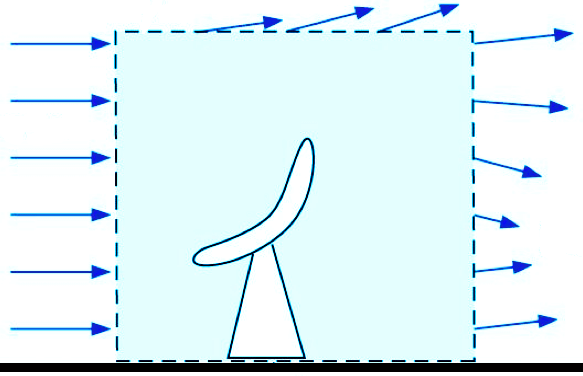
\includegraphics[height = 30mm]{telescope_indirect_blue.png}}
	\end{picture}
\end{itemize}

\vspace{40mm}
\end{frame}



%-----------------------------------------------------------------------------------------
\subsubsection{Théorème d'Euler}
%-----------------------------------------------------------------------------------------
\begin{frame}{Théorème d'Euler}
%-----------------------------------------------------------------------------------------

\small

Rappel  (chapitre 5) :

Soit $\Omega$ un volume de contrôle (fixe) dans le fluide. On note $\partial \Omega$ la frontière du volume de contrôle $\Omega$, et $\myvec{n}$ sa normale sortante.


\pause \medskip

Le bilan intégral de quantité de mouvement pour le fluide contenu dans $\Omega$ est donné par~:
\begin{equation}
   \dpdt{} \int_\Omega \rho \myvec{u} \, dV  
   + \oint_{\partial \Omega} \rho \myvec{u} \left ( \myvec{u} \cdot \myvec{n} \right ) \, dS
   =
    \oint_{\partial \Omega}  ( - p \myvec{n} + \mytensor{\tau} \cdot \myvec{n}) \, dS
   + \int_\Omega \rho \myvec{f} \, dV
\end{equation}



%\pause 
%Ce théorème fournit un outil puissant pour estimer la force $ \myvec{F}$ exercée par un fluide sur un objet si l'on connait (ou si l'on peut modéliser) les champs de vitesse et de pression aux frontières d'un volume de contrôle judicieusement choisi.


\pause
\smallskip

Supposons que la frontière $\partial \Omega = \Sigma \cup \Gamma$ est composée de deux parties :

\begin{itemize}
\item Une surface $\Sigma$ qui est la paroi d'un solide sur lequel le fluide exerce une force 
$\myvec{F}$ que l'on cherche à déterminer 

(et sur laquelle la répartition de pression et de contrainte visqueuse ne sont pas connues).

\item Une surface $\Gamma$ sur laquelle on connait (ou bien on peut modéliser) le champ de pression et de vitesse, et sur laquelle les effets visqueux peuvent être négligés
\end{itemize}

Alors le bilan de quantité de mouvement prend la forme suivante, appelée {\em Théorème d'Euler} :

\begin{equation}
	\color{rouge}
	\myvec{F} 
	=   
  - \oint_{\Gamma} \left[ \rho \myvec{u} \left ( \myvec{u} \cdot \myvec{n} \right) + p \myvec{n} \right] \, dS
%   + \int_{\partial \Omega\backslash \Sigma} \mytensor{\sigma} \cdot \myvec{n} \, dS
   + \int_\Omega \rho \myvec{f} \, dV
\end{equation}

\pause

Utilité : dans de nombreux cas il est possible de séparer $\Gamma$ en plusieurs parties sur lesquelles $p$ et $\myvec{u}$ sont supposés uniformes.

Remarque :
on peut aussi écrire l'intégrale surfacique sous la forme
$- \oint_{\Gamma} \mytensor{\cal D} \cdot \myvec{n}  \, dS$ où $\mytensor{\cal D}  = p \mytensor{1} + \rho \myvec{u} \otimes \myvec{u} $ est le {\em tenseur dynalpie}.


%Remarque : 

%Dans de nombreux cas, il est possible, sous certaines approximations (écoulement stationnaire, etc.), de déterminer les différents termes de droite et ainsi de déterminer indirectement la force exercée par le fluide sur le système, \textcolor{vert}{sans avoir à calculer l'écoulement dans tout le domaine} mais en concentrant l'analyse sur les conditions limites à la frontière du volume de contrôle $\Omega$.

\vspace{0mm}

\end{frame}

%-----------------------------------------------------------------------------------------
\subsubsection{Applications}
%-----------------------------------------------------------------------------------------
\begin{frame}{Théorème d'Euler : Exemples d'applications}
%-----------------------------------------------------------------------------------------

\small

\begin{itemize}
%\item
%  Force de frottement exercée sur une portion de conduite de longueur $L$ 
%  par un écoulement de Poiseuille (cf. section précédente).	



\item
	Force exercée par  l'écoulement dans une conduite coudée.
	
	\item
	Force exercée par l'écoulement dans une conduite avec rétrécissement ou élargissement.

	\item
	Jet impactant sur un auget (TP) ou sur une plaque (ex. 8.2)
\item
	Détermination de la poussée d'un réacteur.
	
\item (...)	

\end{itemize}

\vspace{30mm}

\end{frame}


\comment{
%\end{document}


%-----------------------------------------------------------------------------------------
\subsubsection{Limitations}
%-----------------------------------------------------------------------------------------
\begin{frame}{Détermination directe : limitations}
%-----------------------------------------------------------------------------------------

\small

\begin{itemize}[<+->]
\item[]
	Cette méthode nécessite la connaissance du champ de vitesse et de pression 
	au moins dans le voisinage de la paroi du système
	\medskip
\item[] 
	$\rightarrow$ pas toujours possible !
	\\
	\begin{picture}(0, 0)(-5, 51)
		\put(0, 0){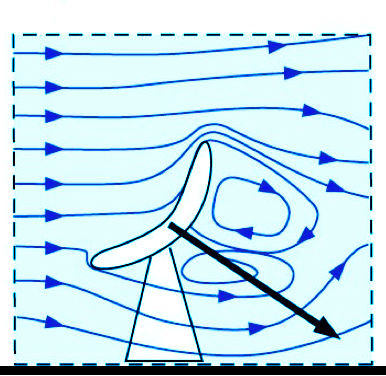
\includegraphics[height = 30mm]{telescope_direct_blue.png}}
	\end{picture}
\item[]
	Alternative ? 
	\medskip
\item[]
	$\rightarrow$ Oui avec un bilan intégral de quantité de mouvement dans un volume de contrôle 
	\mytabbing{$\rightarrow$} bien choisi\ldots
	\\
	\begin{picture}(0, 0)(-50, 35)
		\put(0, 0){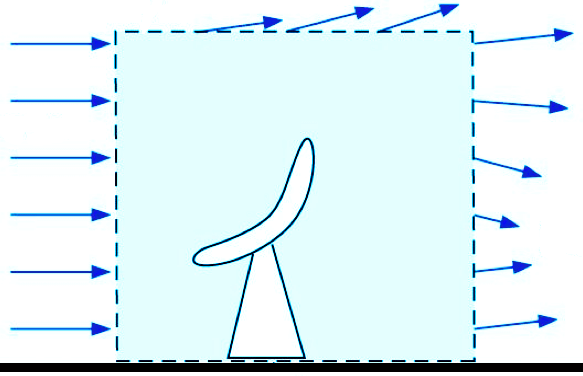
\includegraphics[height = 30mm]{telescope_indirect_blue.png}}
	\end{picture}
\end{itemize}

\vspace{40mm}

\end{frame}
%-----------------------------------------------------------------------------------------
\begin{frame}{Théorème d'Euler}
%-----------------------------------------------------------------------------------------



\end{frame}


%-----------------------------------------------------------------------------------------
\begin{frame}{Théorème d'Euler : applications}
%-----------------------------------------------------------------------------------------



\end{frame}




%%%%%%%%%%%%%%%%%%%%%%%%%%%%%%%%%%%%%%%%%%%%%%%%%%%%%%%%%%%%%%%%%%%%%%%%%%%%%%%%%%%%%%%%%%%
\end{document}
%%%%%%%%%%%%%%%%%%%%%%%%%%%%%%%%%%%%%%%%%%%%%%%%%%%%%%%%%%%%%%%%%%%%%%%%%%%%%%%%%%%%%%%%%%%

%-----------------------------------------------------------------------------------------
\subsubsection{Applications}
%-----------------------------------------------------------------------------------------
\begin{frame}{Applications}
%-----------------------------------------------------------------------------------------

\small

\vspace{0mm}

\end{frame}

%==========================================================================================
\subsection{La couche limite}
%=========================================================================================

%-----------------------------------------------------------------------------------------
\subsubsection{Phénoménologie}
%-----------------------------------------------------------------------------------------
\begin{frame}{Phénoménologie}
%-----------------------------------------------------------------------------------------

\small

\vspace{0mm}

\end{frame}

%-----------------------------------------------------------------------------------------
\subsubsection{Equations de couche limite}
%-----------------------------------------------------------------------------------------
\begin{frame}{Equations de couche limite}
%-----------------------------------------------------------------------------------------

\small

\vspace{0mm}

\end{frame}

%-----------------------------------------------------------------------------------------
\subsubsection{Conséquences physiques ?}
%-----------------------------------------------------------------------------------------
\begin{frame}{Conséquences physiques ?}
%-----------------------------------------------------------------------------------------

\small

\vspace{0mm}

\end{frame}


%-----------------------------------------------------------------------------------------
\subsubsection{Conditions aux limites}
%-----------------------------------------------------------------------------------------
\begin{frame}{Conditions aux limites}
%-----------------------------------------------------------------------------------------

\small

	\begin{center}
		\setlength{\unitlength}{0.7mm}
		\begin{picture}(65, 50)(12, -12)
			\put(0, 0){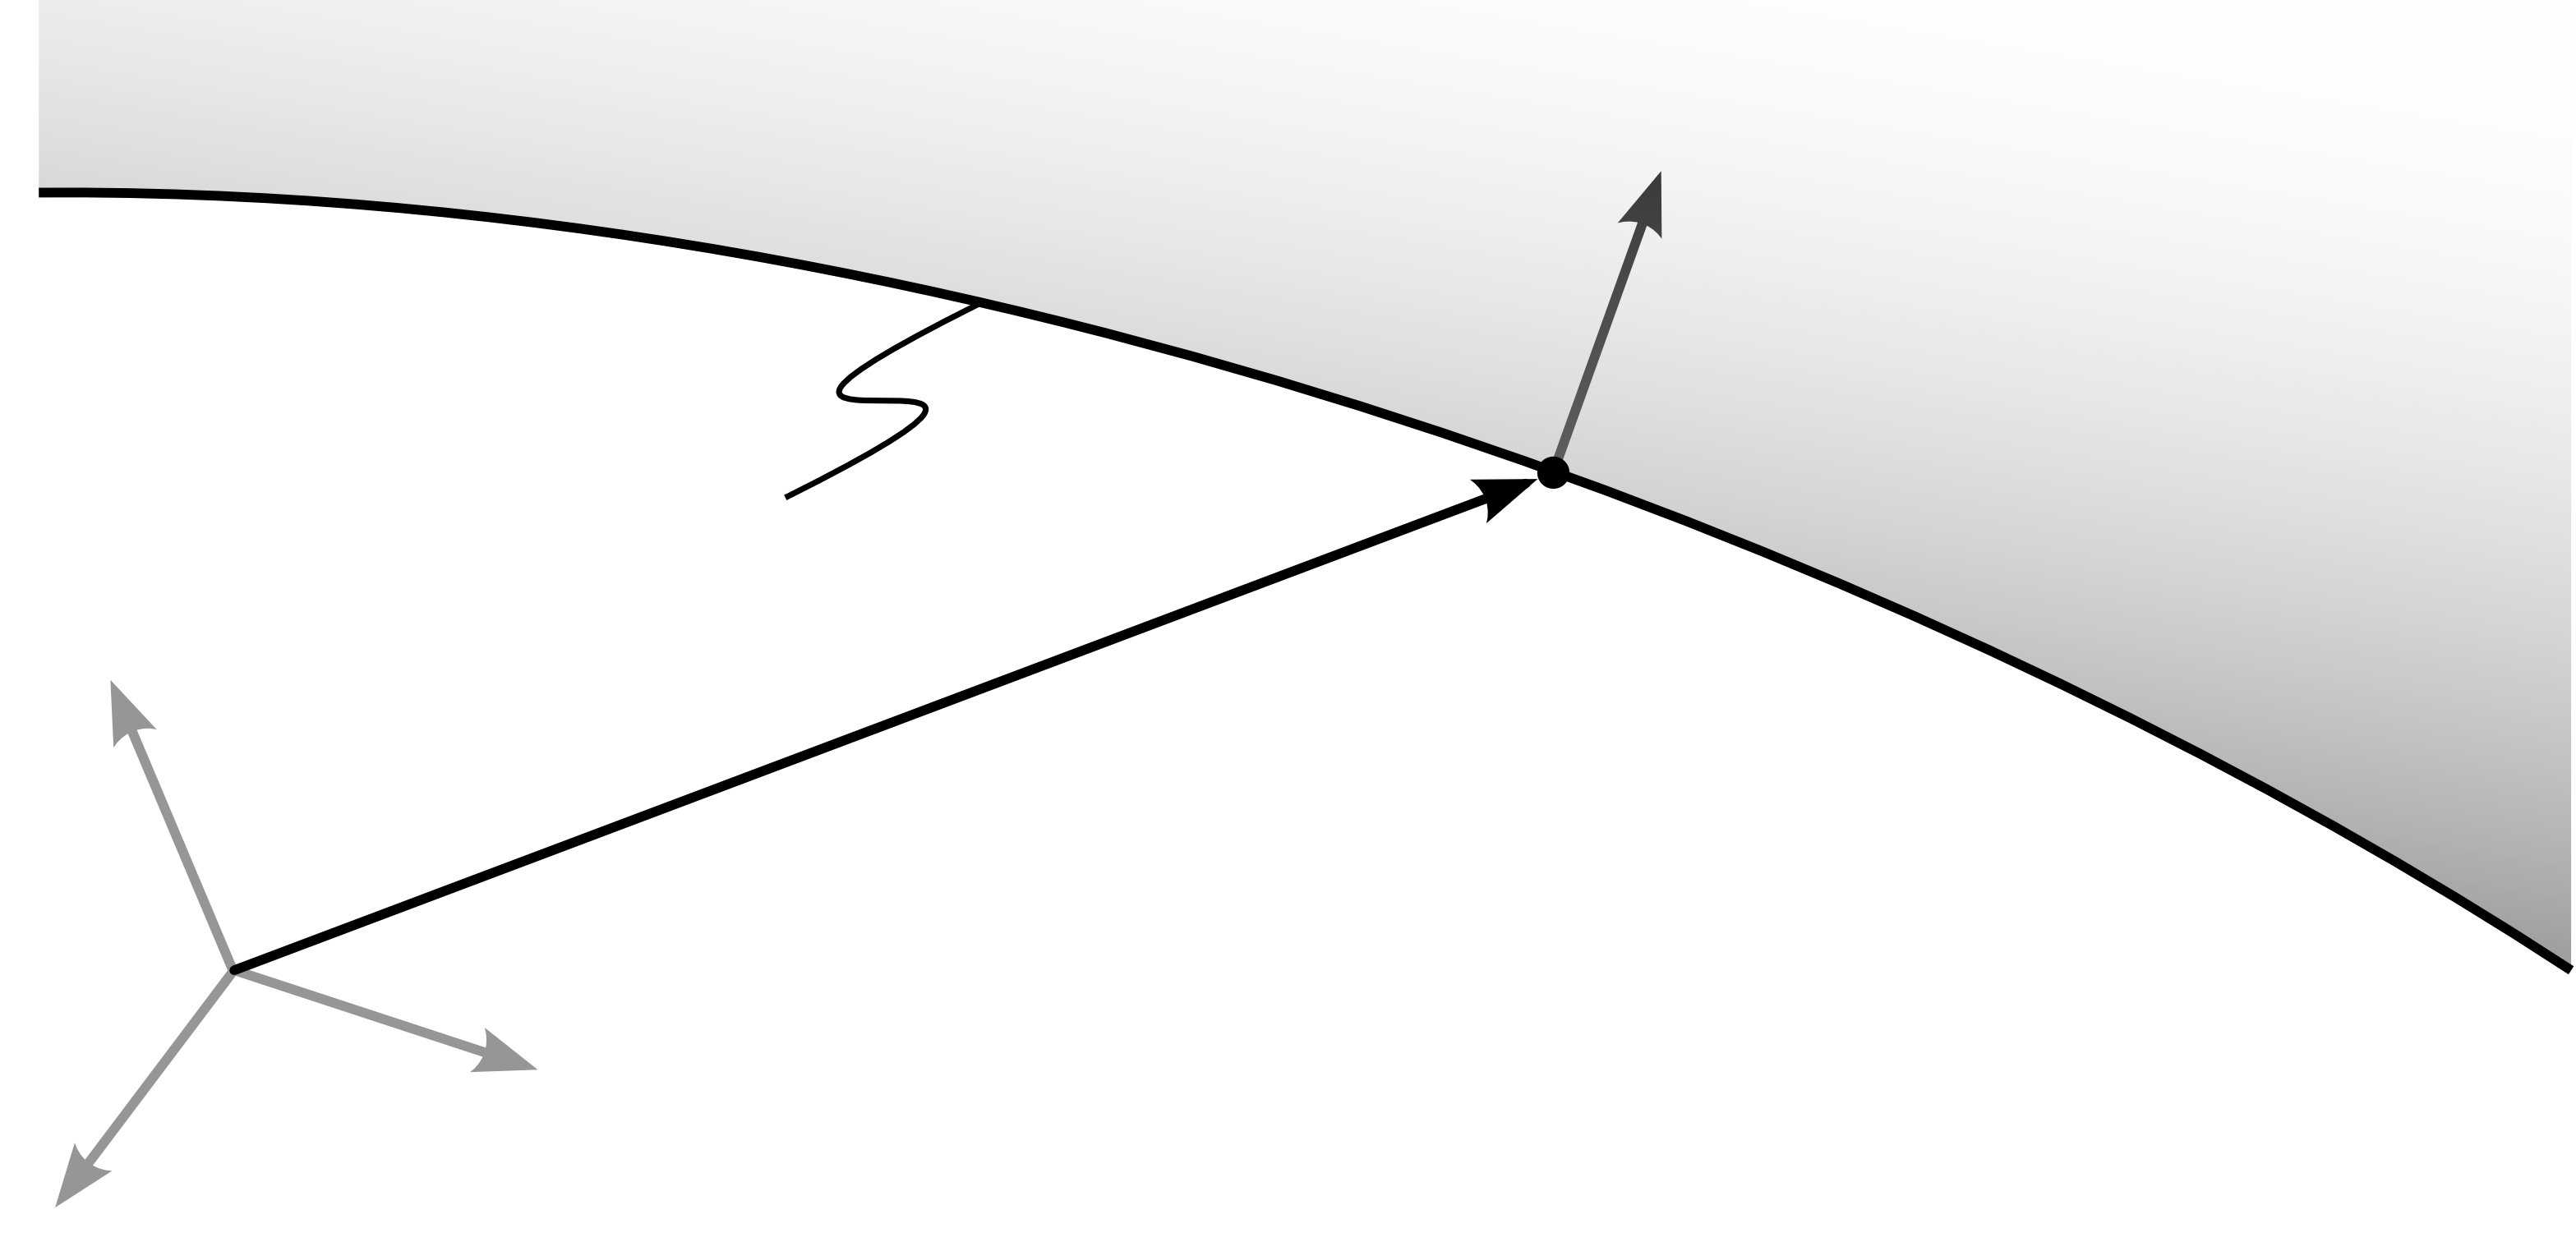
\includegraphics[width=63mm]{conditions_limites.png}}	
			\put(58, 39){$\myvec{n}$}
			\put(63.5, 32){milieu extérieur}
			\put(63, 27){(fluide ou solide)}
			\put(28, 17){\setlength{\fboxsep}{1mm}\colorbox{white}{$\myvec{x}$}} 
			\put(9, 24){\color{rouge} frontière $\Sigma$}
			\put(63, 15){fluide}
		\end{picture}
	\end{center}

\pause

\vspace{-8mm}

\begin{tabular}{cll}
& 
\bf condition cinématique :
& 
\bf condition dynamique :
\\ & & \\
fluide réel 
&
continuité de la vitesse
&
continuité des contraintes
\\
(visqueux) & &
\\
&
$\color{bleu}\myvec{u}(\myvec{x} \in \Sigma, t) = \myvec{u}\indice{ext}(\myvec{x} \in \Sigma, t)$
&
$\color{bleu}	\mytensor{\sigma}(\myvec{x} \in \Sigma, t) \cdot \myvec{n} 
	= 
	\mytensor{\sigma}\indice{ext}(\myvec{x} \in \Sigma, t)\cdot \myvec{n}$
	\pause
\\ & \hspace{15mm}\vector(0, -1){5} & \hspace{15mm}\vector(0, -1){5} \\ & & \\
\color{rouge} 
fluide parfait 
&
continuité de la vitesse \textcolor{rouge}{normale}
&
continuité de la \textcolor{rouge}{pression}
\\
(non visqueux) & &
\\
&
$\color{bleu}\myvec{u}(\myvec{x} \in \Sigma, t){\color{rouge}\cdot \myvec{n} }
= 
\myvec{u}\indice{ext}(\myvec{x} \in \Sigma, t){\color{rouge}\cdot  \myvec{n}}$
&
$\color{rouge}p(\myvec{x} \in \Sigma, t) = p\indice{ext}(\myvec{x} \in \Sigma, t)$

\end{tabular}

\pause

\bigskip
$\longrightarrow$
En particulier si $\Sigma$ correspond à une paroi solide, il n'y a plus adhérence mais
\textcolor{vert}{glissement}.

\vspace{0mm}

\end{frame}
}
